\scanpage{86}
% archive foliation: 85
% lines 1--3
Soit $\unsure{\mathcal T|\Gamma}_\nu^{!}$ le ss-groupe de $\unsure{\mathcal T|\Gamma}_\nu$
formé des éléments qui satisfont
aux relations précédentes. Donc\ldots
% lines 4--7
\diagram{\begin{tikzcd}[ampersand replacement=\&]
1\arrow[r,dash]\&\unsure{\mathcal T|\Gamma}_\nu^{!0}\arrow[r,dash]\&\unsure{\mathcal T|\Gamma}_\nu^{!}\arrow[r]\&\widehat{\mathbb Z}^{\times}\arrow[r,dash]\&1
\end{tikzcd}}
avec
\[
\begin{aligned}
\unsure{\mathcal T|\Gamma}_\nu^{!0}&\subset\unsure{\mathcal T|\Gamma}_\nu^{0}\\
\Vert\qquad&\\[-1ex]
\{\gamma\in\unsure{\mathcal T|\Gamma}_\nu^0\mid\gamma&\text{ commute aux }\rho_\nu(i)\\
&\text{et à }t_\nu\}
\end{aligned}
\]
\figure{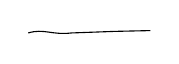
\begin{tikzpicture}\draw (0,0) .. controls (.2,.06) and (.3,-.03) .. (.55,0) -- (1.1,.02) -- (1.55,.03);\end{tikzpicture}}
% lines 8--11
Si $\nu=2$ il y a un autre choix
intéressant de $\unsure{I_0|I}\subset\mathbb P^1(\overline Q)$, savoir
\[
I=\{0,1,\infty\}\qquad(\text{plutôt que }I=\mu_3(\overline Q))
\]
% lines 12--15
qui donne lieu à action de
$\unsure{\mathfrak S_3|\mathcal S_3}$ sur $(X_0/I_0/k)$ -- on trouve
action de $\Gamma\times\unsure{\mathfrak S_3|\mathcal S_3}\,\unsure{\times}$ sur $F_2^{ext}$, i.e.
\[
\Gamma\times\unsure{\mathfrak S_3|\mathcal S_3}\longrightarrow\widetilde{\unsure{\mathcal T|\Gamma}}_2
\]
